\documentclass[a4paper,14pt]{extreport} % формат документа

\usepackage{amsmath}
\usepackage{cmap} % поиск в ПДФ
\usepackage[T2A]{fontenc} % кодировка
\usepackage[utf8]{inputenc} % кодировка исходного текста
\usepackage[english,russian]{babel} % локализация и переносы
\usepackage[left = 2cm, right = 1cm, top = 2cm, bottom = 2 cm]{geometry} % поля
\usepackage{listings}
\usepackage{graphicx} % для вставки рисунков
\usepackage{amsmath}
\usepackage{float}
\usepackage{multirow}
\graphicspath{{pictures/}}
\DeclareGraphicsExtensions{.pdf,.png,.jpg}
\newcommand{\anonsection}[1]{\section*{#1}\addcontentsline{toc}{section}{#1}}

\lstset{ %
	language=Lisp,                % Язык программирования 
	numbers=left,                   % С какой стороны нумеровать          
	frame=single,                    % Добавить рамку
}

\begin{document}
\begin{titlepage}

    \begin{table}[H]
        \centering
        \footnotesize
        \begin{tabular}{cc}
            \multirow{8}{*}{
\includegraphics[scale=0.35]{bmstu.jpg}}
            & \\
            & \\
            & \textbf{Министерство науки и высшего образования Российской Федерации} \\
            & \textbf{Федеральное государственное бюджетное образовательное учреждение} \\
            & \textbf{высшего образования} \\
            & \textbf{<<Московский государственный технический} \\
            & \textbf{университет имени Н.Э. Баумана>>} \\
            & \textbf{(МГТУ им. Н.Э. Баумана)} \\
        \end{tabular}
    \end{table}

    \vspace{-2.5cm}

    \begin{flushleft}
        \rule[-1cm]{\textwidth}{3pt}
        \rule{\textwidth}{1pt}
    \end{flushleft}

    \begin{flushleft}
        \small
        ФАКУЛЬТЕТ
        \underline{<<Информатика и системы управления>>\ \ \ \ \ \ \ 
        \ \ \ \ \ \ \ \ \ \ \ \ \ \ \ \ \ \ \ \ \ \ \ \ \ \ \ \ \ \ \ 
    \ \ \ \ \ \ \ \ \ \ \ \ \ \ \ } \\
        КАФЕДРА
        \underline{<<Программное обеспечение ЭВМ и
        информационные технологии>>
        \ \ \ \ \ \ \ \ \ \ \ \ \ \ \ \ \ \ \ \ }
    \end{flushleft}

    \vspace{2cm}

    \begin{center}
        \textbf{Лабораторная работа № 7} \\
        \vspace{0.5cm}
        \textbf{} \\
    \end{center}

    \vspace{4cm}

    \begin{flushleft}
        \begin{tabular}{ll}
            \textbf{Дисциплина} & Функциональное и логическое программирование \\
            \textbf{Студент} & Сиденко А.Г. \\
            \textbf{Группа} & ИУ7-63Б \\
            \textbf{Преподаватель} & Толпинская Н.Б., Строганов Ю.В.  \\
        \end{tabular}
    \end{flushleft}

    \vspace{4cm}

   \begin{center}
        Москва, 2020 г.
    \end{center}

\end{titlepage}

\begin{enumerate}
\item \textbf{Написать предикат, который принимает два числа-аргумента и возвращает Т, если первое число не меньше второго.}

\begin{lstlisting}
(defun eqb (a b)
  (if (> b a) Nil T)
)
\end{lstlisting}

\item \textbf{Какой из следующих двух вариантов предиката ошибочен и почему?}

\begin{lstlisting}
(defun pred1 (x)
  (and (numberp x) (plusp x))
)

(defun pred2 (x)
  (and (plusp x) (numberp x))
)
\end{lstlisting}

Ошибочен второй, так как перед выполнением операции, не делается проверка на число. 

\item \textbf{Переписать функцию how-alike, приведенную в лекции и не пользующую COND, используя конструкция IF, AND/OR.}

\begin{lstlisting}
(defun how_alike (x y)
  (cond 
    ((or (= x y) (equal x y)) 'the_same)
    ((and (oddp x) (oddp y)) 'both_odd)
    ((and (evenp x) (evenp y)) 'both_even)
    (T 'difference)
  ) 
)

(defun how_alike_if (x y)
  (if (or (= x y) (equal x y)) 'the_same
    (if (and (oddp x) (oddp y)) 'both_odd
      (if (and (evenp x) (evenp y)) 'both_even 
        'difference
      )
    )
  ) 
)
\end{lstlisting}

Результат:

(how$\_$alike 11 30) $\to$ DIFFERENCE

(how$\_$alike$\_$if 11 30) $\to$ DIFFERENCE

(how$\_$alike 3 3) $\to$ THE$\_$SAME

(how$\_$alike$\_$if 3 3) $\to$ THE$\_$SAME

(how$\_$alike 1 3) $\to$ BOTH$\_$ODD

(how$\_$alike$\_$if 1 3) $\to$ BOTH$\_$ODD

(how$\_$alike -2 30) $\to$ BOTH$\_$EVEN

(how$\_$alike$\_$if -2 30) $\to$ BOTH$\_$EVEN

\item \textbf{Чем принципиально отличаются функции cons, list, append?}

(cons lst1 lst2) $\to$ ((1 2 3) 4 5)

(list lst1 lst2) $\to$ ((1 2 3) (4 5))

(append lst1 lst2) $\to$ (1 2 3 4 5)

CONS -- позволяет создавать списки (возвращает бинарную ячейку (точечная пара, список), расставляя указатели, обязательно 2 аргумента). 

APPEND -- функция двух аргументов x и y, сцепляющая два списка в один.

LIST -- создает столько списковых ячеек, сколько аргументов (всегда возвращает список).

\item \textbf{Каковы результаты вычисления следующих выражений?}

(reverse ()) $\to$ Nil

(last ()) $\to$ Nil

(reverse '(a)) $\to$ (a)

(last '(a)) $\to$ (a)

(reverse '((a b c))) $\to$ ((a b c))

(last '((a b c))) $\to$ ((a b c))

\item \textbf{Написать, по крайней мере, два варианта функции, которая возвращает последний элемент своего списка-аргумента.}

Рекурсивно -- пока второй элемент не Nil идем дальше, иначе возвращаем голову:

\begin{lstlisting}
(defun last_elem (lst)
  (if (NULL (cadr lst)) (car lst) 
    (last_elem (cdr lst))
  ) 
)
\end{lstlisting}

С использованием функционала -- с использованием функционала reduce, возвращая последний полученный результат, а возвращаем каждый раз второй аргумент:

\begin{lstlisting}
(defun last_elem (lst)
  (reduce #'(lambda (a x) x) lst)
)
\end{lstlisting}

\item \textbf{Написать, по крайней мере, два варианта функции, которая возвращает свой список-аргумент без последнего элемента.}

С использованием функционала -- пользуясь тем, что mapcar будет работать до хвоста в самом коротком списке (cdr lst всегда на один короче lst), возвращаем значение из lst, таким образом получится список без последнего элемента:

\begin{lstlisting}
(defun centr (lst)
  (mapcar (lambda (x y) y) (cdr lst) lst)
)
\end{lstlisting}

Рекурсивно -- пока хвост не Nil, соединяем с помощью cons голову и возвращаем значение функции от хвоста:

\begin{lstlisting}
(defun centr (lst)
  (if (NULL (cadr lst)) () 
    (cons (car lst) (centr (cdr lst)))
  )
)
\end{lstlisting}

\item \textbf{Написать простой вариант игры в кости, в котором бросаются две правильные кости. Если сумма выпавших очков равна 7 или 11 -- выигрыш, если выпало (1,1) или (6,6) --- игрок право снова бросить кости, во всех остальных случаях ход переходит ко второму игроку, но запоминается сумма выпавших очков. Если второй игрок не выигрывает абсолютно, то выигрывает тот игрок, у которого больше очков. Результат игры и значения выпавших костей выводить на экран с помощью функции print.}

Функция game запускает игру, в которой анализируются 2 рандомных числа (от 1 до 6) для 2 игроков. Далее сравниваются их суммы, в зависимости от этого возвращается результат. 

Функция analyze принимает на вход 2 числа, и в зависимости от них, либо перекидывает кости (функция вызывается еще раз с новыми параметрами) либо возвращает число (сумму очков). 

Функция printS выводит очки и их сумму на экран. 

\begin{lstlisting}
(defun printS (x y s)
  (print (list x '+ y '= s))
)

(defun analyze (x y)
  (cond 
    ((and (= 1 x) (= 1 y)) (printS x y (+ x y)) 
        (analyze (+ 1 (random 6)) (+ 1 (random 6))))
    ((and (= 6 x) (= 6 y)) (printS x y (+ x y))
        (analyze (+ 1 (random 6)) (+ 1 (random 6))))
    (T (printS x y (+ x y)) (+ x y))
  ) 
)

(defun game ()
  (let ((s1 (analyze (+ 1 (random 6)) (+ 1 (random 6))))
        (s2 (analyze (+ 1 (random 6)) (+ 1 (random 6)))))
    (cond 
      ((or (= s1 7) (= s1 11) (> s1 s2)) 'you-win)
      ((or (= s1 7) (= s2 11) (< s1 s2)) 'he-wins)
      (T 'draw)
    )
  )
)
\end{lstlisting}

\hfill

Примеры работы:

\begin{figure}[ht]\center
	\begin{tabular}{cc}
		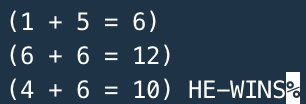
\includegraphics[width=80mm]{1} & 
\includegraphics[width=80mm]{2} \\
		
\includegraphics[width=80mm]{3} & 
\includegraphics[width=80mm]{4}
	\end{tabular}
\end{figure}


\includegraphics[width=80mm]{5}

\end{enumerate}
\end{document}